\subsection{タイトル}

表\ref{table:title}に示すコマンドを使えば,レポートなどのタイトルを簡単に作成することができる.まず,\verb|\title{}|,\verb|\author{}|,\verb|\date{}|コマンドを使ってタイトル・著者名・日付を指定したあと,\verb|\maketitle|コマンドを実行してタイトルを出力する.

\begin{table}[h]
    \caption{タイトルに関するコマンド}
    \label{table:title}
    \centering
    \begin{tabular}{c|c}
        コマンド & 内容 \\ \hline
        \verb|\title{}| & タイトルの指定 \\
        \verb|\author{}| & 著者名の指定 \\
        \verb|\date{}| & 日付の指定 \\
        \verb|\maketitle| & タイトル・著者名・日付の出力
    \end{tabular}
\end{table}

例えば,
\begin{screen}
\begin{verbatim}
\title{情報実習Iレポート}
\author{情報太郎}
\date{2019年5月1日}
\maketitle
\end{verbatim}
\end{screen}
とソースファイルに書けば,
% \maketitle コマンドでは意図したとおりに出力できないので,
% 他のコマンドを使って模擬している.
\begin{screen}
\begin{center}
{\Large 情報実習Iレポート}\\
 \\
情報太郎\\
 \\
2019年5月1日
\end{center}
\end{screen}
と出力される.なお,タイトル作成については次の点も留意しておくと良い.
\begin{itemize}
\item タイトル・著者名が長くなってしまった場合は \verb|\\| で強制改行して見やすくすると良い(\ref{sec:return}節参照).例えば,\verb|\title{タイトルの一行目 \\ タイトルの二行目}|のように書く.
\item 著者が複数いる場合は,\verb|\and| コマンドで区切って記述する.例えば \verb|\author{情報太郎 \and 近大花子}|のように書く.
\item 日付を指定するときには \verb|\today| という特別なコマンドがあり,\verb|\date{\today}| とすればタイプセットを行った日が自動的に指定される.
\end{itemize}

\subsection{節番号}
\label{sec:section}

レポートなどの技術文書ではその構造が重要になる.文書の構造については教科書\cite{TeXText}の第3章の3.1節で説明されているのでそちらを参照すること.文書の構造を分かりやすく示すために,表\ref{table:section}に示すコマンドを使って階層的な見出しをつける.

表\ref{table:section}に示すコマンドはいつでも利用できるわけではなく,作成している文書のスタイルによって利用可能なコマンドが決まる.例えば,「部」「章」は書籍のような大規模な文書を執筆する際に利用し,レポートなどの場合には使用しない.当面は \verb|\section{}| や \verb|\subsection{}| を中心に使用し,もし必要があればさらに細かな階層のコマンドを用いるようにする.

\begin{table}[t]
    \caption{階層的な見出しを付けるためのコマンド}
    \label{table:section}
    \centering
    \begin{tabular}{c|c}
        コマンド & 内容 \\ \hline
        \verb|\part{}| & 部 \\
        \verb|\chapter{}| & 章 \\
        \verb|\section{}| & 節 \\
        \verb|\subsection{}| & 小節(項)\\
        \verb|\subsubsection{}| & 小小節(目)\\
        \verb|\paragraph{}| & 段落\\
        \verb|\subparagraph{}| & 小段落\\
    \end{tabular}
\end{table}

もちろん,この文書自体も \verb|\section{}| や \verb|\subsection{}| を使用している.例えば,\ref{sec:command_reference}節の見出しを付けるためには
\begin{screen}
\begin{verbatim}
\section{コマンドリファレンス}
\end{verbatim}
\end{screen}
と,\ref{sec:section}節の見出しを付けるためには,
\begin{screen}
\begin{verbatim}
\subsection{節番号}
\end{verbatim}
\end{screen}
とソースファイルに記述している.このように,節や小節の見出しのみを記述すれば,\LaTeX が連番を割り当ててくれる.

\subsection{表の作成}
\label{sec:table}

実験や調査の結果を分かりやすく示すため表を用いると良い場合がある.表の作成のため多くのコマンドが用意されており,それらを駆使すると複雑な表を作成できるが,まずは単純なものをマスターするようにすれば良い.

まず,簡単な例を以下に示す.
\begin{screen}
\begin{verbatim}
\begin{table}[!h]
\caption{lsコマンドの使い方と実行結果}
\label{tab:ls}
\begin{center}
\begin{tabular}{|c||c|}\hline
コマンド & 実行結果 \\ \hline
\verb*|ls| & カレントディレクトリのファイル一覧を表示 \\ \hline
\verb*|ls ー l| & ``説明'' \\ \hline
\verb*|ls - al| & ``説明'' \\ \hline
\end{tabular}
\end{center}
\end{table}
\end{verbatim}
\end{screen}
のようにソースファイルに記述すると,表\ref{tab:ls}のような表が出力される.
\begin{table}[!h]
\caption{lsコマンドの使い方と実行結果}
\label{tab:ls}
\begin{center}
\begin{tabular}{|c||c|}\hline
コマンド & 実行結果 \\ \hline
\verb*|ls| & カレントディレクトリのファイル一覧を表示 \\ \hline
\verb*|ls ー l| & ``説明'' \\ \hline
\verb*|ls - al| & ``説明'' \\ \hline
\end{tabular}
\end{center}
\end{table}
これを順を追って説明していく.
\begin{itemize}
    \item 最初の行の \verb|\begin{table}| と最後の行の \verb|\end{table}| の対で \verb|table| 環境を使ってる.\verb|table| 環境は表の配置を決め,その中に見出しや表の本体を記述する.

    \item \verb|\begin{table}| のあとについている \verb|[!h]| は表の配置を指定するオプションである.配置を指定するオプションには表\ref{table:position}のような種類がある.これらは複数指定することができ,最初に指定した方が優先される.例えば \verb|htbp| と指定すれば,まず \verb|h| による配置が試みられ,うまく配置できなければ次に \verb|t| という順に処理が行われる.表や図を配置する場合は,文章中の図表の割合などの基準と照らし合わせて \LaTeX が適切な場所を選択するので,必ずしもユーザーの指定通りにはいかない.特に最初はもどかしい思いをすることもあるが,\ref{sec:cross_reference}節で述べる相互参照が正しく行われていれば,まずは問題ないと考えて良い.
    \item \verb|\caption{}| は表の見出しを指定する.表では見出しは表本体の上部に書き,図では見出し
    は図本体の下部に書く.

    \begin{table}[t]

        \caption{表や図の配置を指定するためのオプション}
        \label{table:position}
        \centering
        \begin{tabular}{c|c}
            オプション & 内容 \\ \hline
            \verb|h| & この場所(here) \\
            \verb|t| & ページ上端(top) \\
            \verb|b| & ページ下端(bottom) \\
            \verb|p| & 表や図だけのページを用意してそこに出力 \\
            \verb|!h| & できるだけここに出力\\
        \end{tabular}
    \end{table}

    \begin{table}[t]

        \caption{表中の列の出力形式を指定するためのオプション}
        \label{table:table_column}
        \centering
        \begin{tabular}{c|c}
            オプション & 内容 \\ \hline
            \verb|l| & 項目が左寄せされる列 \\
            \verb|c| & 項目が中央寄せされる列 \\
            \verb|r| & 項目が右寄せされる列 \\
            \verb+|+ & 列と列の間に一本縦線を引く \\
            \verb+||+ & 列と列の間に二本縦線を引く \\
        \end{tabular}
    \end{table}



    \item \verb|\label{}| は相互参照を用いるときに使用するラベルを指定する.詳しくは\ref{sec:cross_reference}節で述べる.
    \item \verb|center|環境は\ref{sec:alignment}節で説明したとおり,中央に揃える環境である.
    \item \verb|\begin{tabular}| と \verb|\end{tabular}| の対に囲まれている \verb|tabular| 環境を用いて表本体を記述する.

    \item \verb|\begin{tabular}| コマンドについているオプション \verb+{|c||c|}+ は表に含まれる列の数と形式を指定している.\verb|c| は項目が中央寄せされる列を,\verb+|+ は列の間の縦線を示している.表\ref{tab:ls}の出力内容と照らし合わせて確認すること.他にも多くのオプションがあるが,代表的なものを表\ref{table:table_column}に示している.
    \item \verb|tabular| 環境の中に記述されているコマンドの意味は次のとおりである.
    \begin{description}
        \item[] \verb+\hline+:横線を出力する
        \item[] \verb+\\+:改行
        \item[] \verb+&+:列の区切り
    \end{description}
    一行に含まれる列の数は冒頭の \verb+\begin{tabular}+ のオプションで指定した列の数に一致しなければならないので注意する.

    \item 表の中に記述されている \verb+\verb||+ と \verb+\verb*||+ は文字をそのまま表示したいときに用いるコマンドである.\verb+||+ に挟まれた文字列がそのまま出力される.\verb+\verb||+ と \verb+\verb*||+ はほぼ同じであるが,後者は半角スペースを \verb*+ + のように明示する

\end{itemize}

\subsection{相互参照}
\label{sec:cross_reference}

\ref{sec:table}節で説明した表や,次の\ref{sec:figure}節で説明する図を挿入したときは,本文の中でもそれについて言及・説明するのが基本である.基本的には,どこからも言及されない図・表は存在しないと考えて欲しい.表や図について言及するときには,これまでの説明でも出てきているように,「表\ref{table:table_column}のように・・・」のような形で,表や図の番号を示して参照する.これは表や図に限った訳ではなく「\ref{sec:table}節で・・・」のように節などにも当てはまる.

表・図・節などを参照するときには,その番号を手入力する必要はなく,自動的に適切な番号を出力する機能が備わっている.そのためには,二つのコマンド \verb|\label{}| と \verb|\ref{}| を対で利用する.まず,\verb|\label{}| を使ってあらかじめ参照先(表・図・節)にラベルを付けておく.例えば\ref{sec:table}節で示したソースファイルでは,

\begin{screen}
\begin{verbatim}
\label{tab:ls}
\end{verbatim}
\end{screen}

として \verb|tab:ls| というラベルをつけている\footnote{ラベルは半角の英字・数字であれば何でもよいが,表は tab:,図は fig: を頭につける,などのルールを設けておけば混乱しなくて良い.}.

ラベルを付けておいたものを参照するときは,
\begin{screen}
\begin{verbatim}
表 \ref{tab:ls} に示すように・・・
\end{verbatim}
\end{screen}
のように \verb|\ref{}| コマンドを用いて記述しておけば,タイプセットを実行するときに自動的に数値に置き換わって,「表 \ref{tab:ls} に示すように・・・」と出力される.

\subsection{図の挿入}
\label{sec:figure}

説明のために必要な模式図や写真は「図」として挿入する.図を挿入するためには様々な方法があるが,ここでは画像ファイル(PNGファイル)を挿入する方法を説明する.

標準では画像ファイルを挿入できないため,追加機能として \verb|graphicx| パッケージを用いて画像ファイルを挿入する.\verb|graphicx| パッケージを利用するためにはプリアンブル(\ref{sec:source}節参照)に
\begin{screen}
\begin{verbatim}
\usepackage[dvipdfmx]{graphicx}
\end{verbatim}
\end{screen}
と記述する.その上で,本文中に次のように記述すれば画像による図が挿入される.
\begin{screen}
\begin{verbatim}
\begin{figure}[!h]
\begin{center}
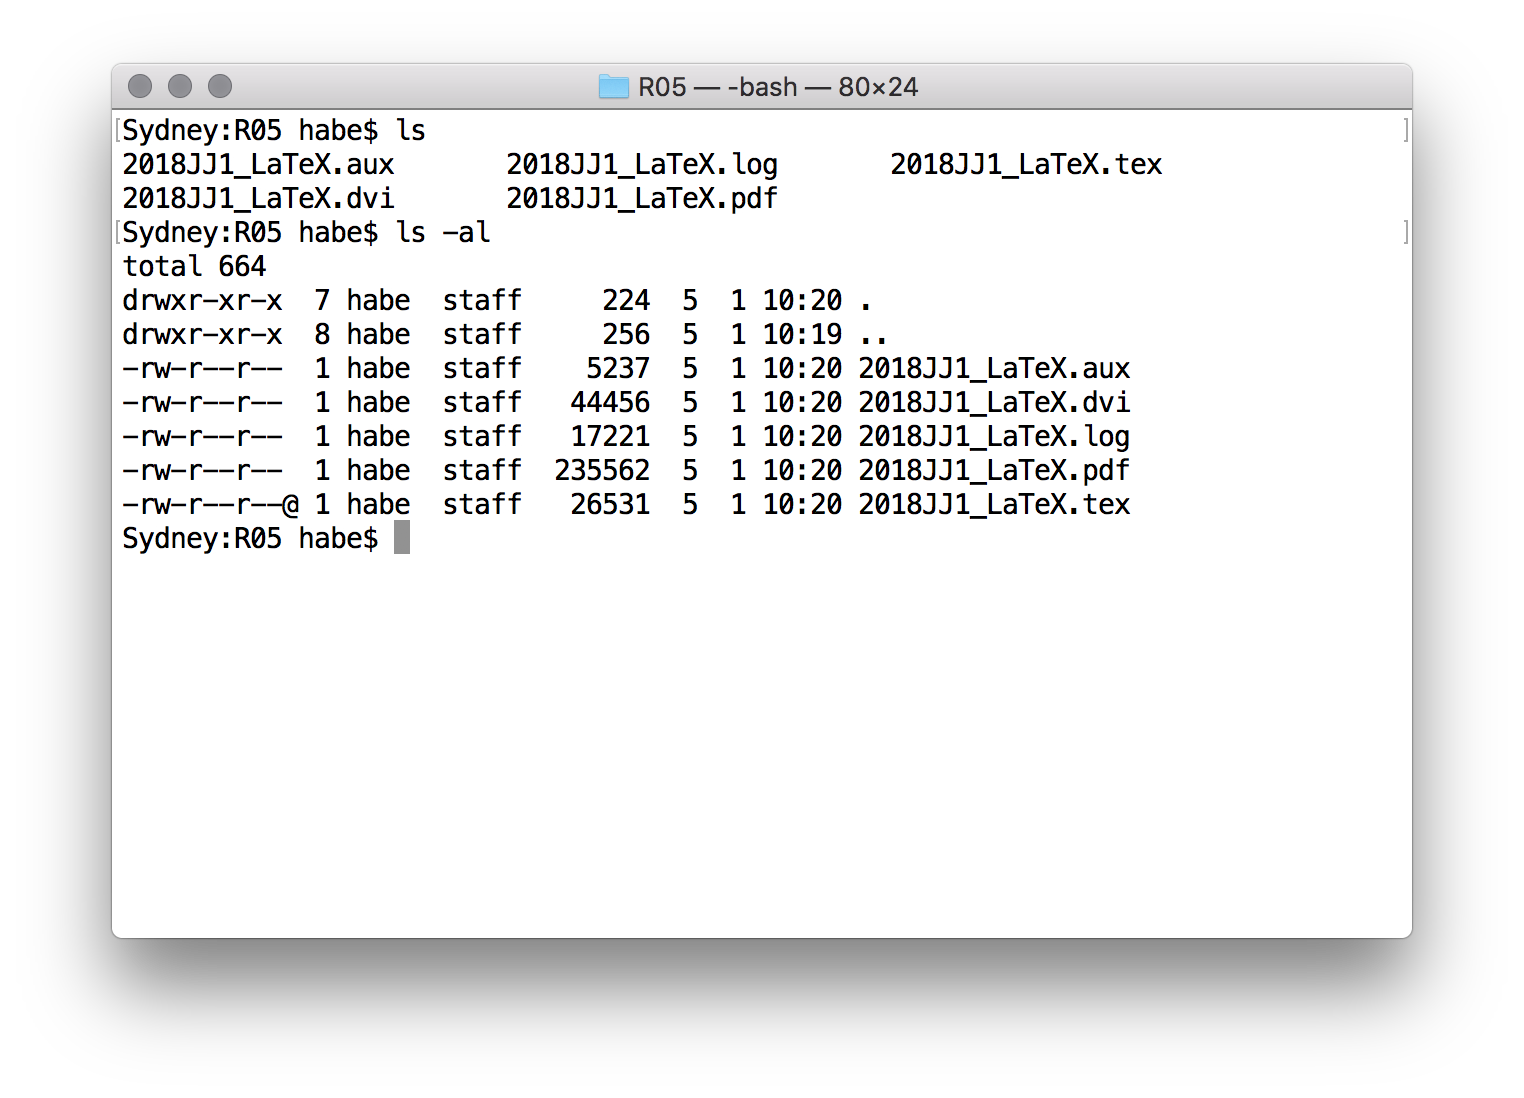
\includegraphics[scale=0.6,clip]{ls.png}
\caption{ls,ls ‐ al コマンド実行の様子}
\label{fig:ls}
\end{center}
\end{figure}
\end{verbatim}
\end{screen}

\begin{figure}[!h]
\begin{center}
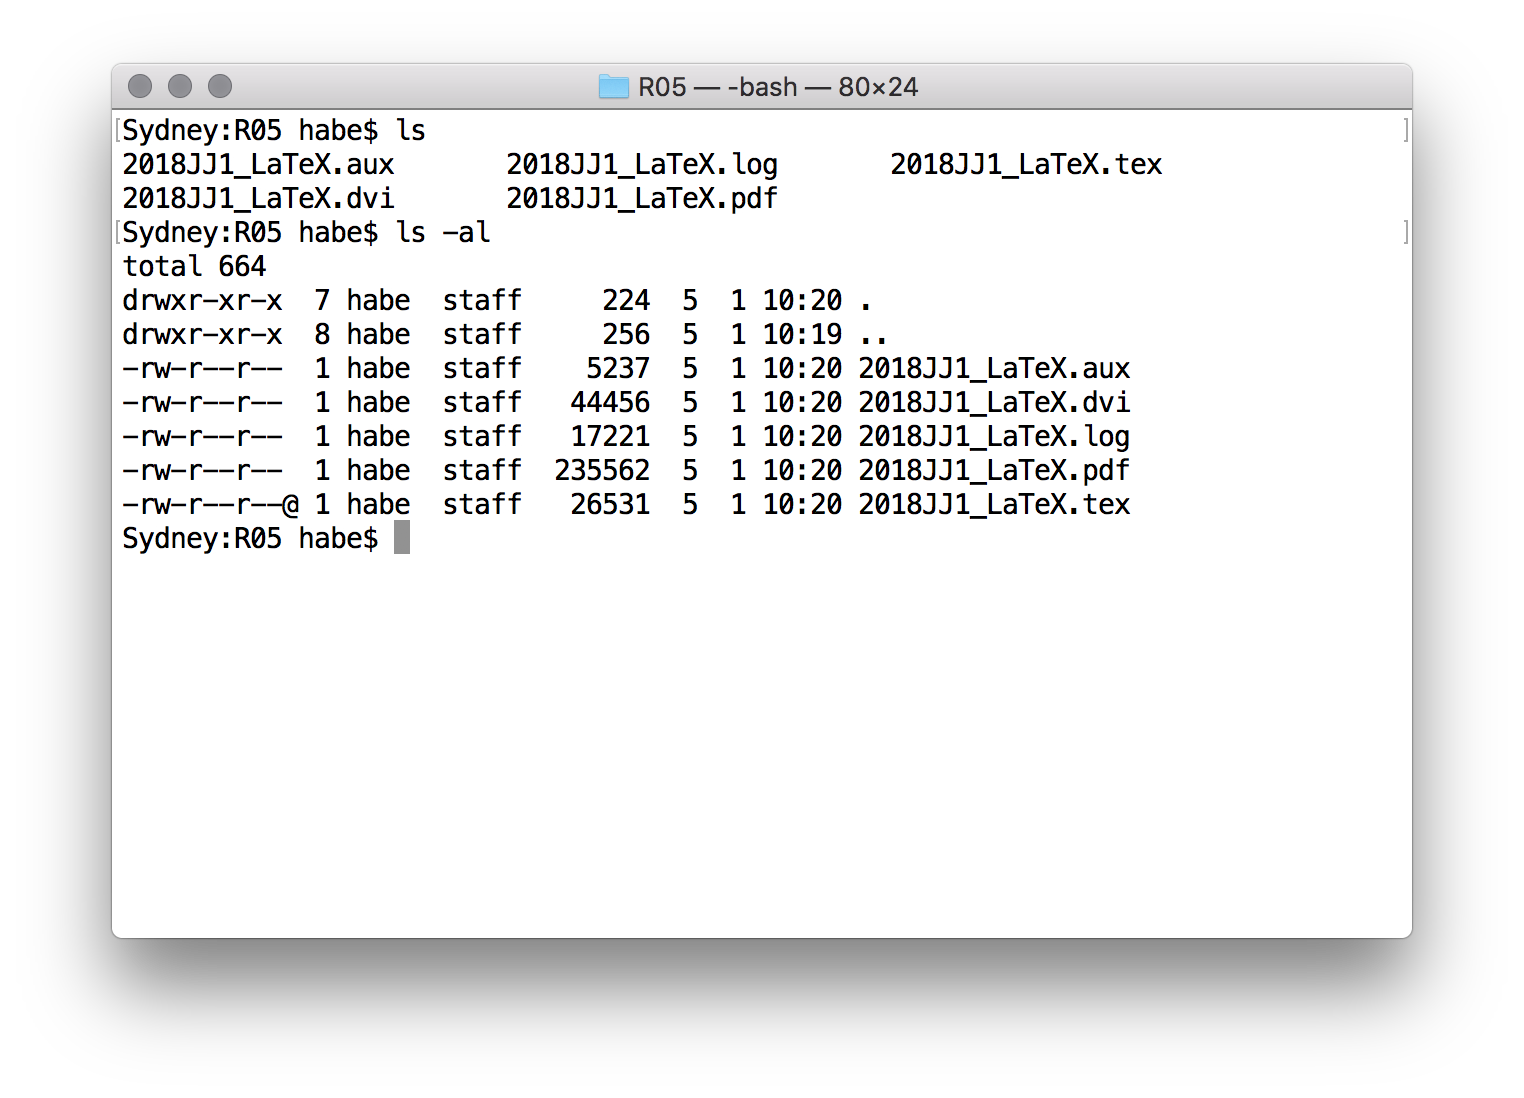
\includegraphics[scale=0.6,clip]{ls.png}
\caption{ls,ls ‐ al コマンド実行の様子}
\label{fig:ls}
\end{center}
\end{figure}

これを順を追って説明していく.
\begin{itemize}
    \item 最初の行の \verb|\begin{figure}| と最後の行の \verb|\end{figure}| の対で \verb|figure| 環境を使ってる.\verb|table| 環境と同じように,図の配置を決め,その中に画像など図の本体や見出しを記述する.

    \item \verb|\begin{figure}| のあとについている \verb|[!h]| は表の配置を指定するオプションである.配置を指定するオプションは表と同じであり,表\ref{table:position}のような種類がある.
    \item \verb|center|環境は\ref{sec:alignment}節で説明したとおり,中央に揃える環境である.
    \item \verb|\includegraphics| が画像を挿入するコマンドである.ここで指定されているオプションの意味は次のとおりである.
    \begin{description}
        \item[] \verb+scale=0.6+:元の画像サイズの0.6倍で出力する.タイプセットしたあとの大きさを確認して適切な数値にすること.小さくて図中の文字が見えないようなことは厳禁である.
        \item[] \verb+clip+:はみ出した分を切り取る.通常は指定しておいた方が良い.
        \item[] \verb+{ls.png}+:\verb+{}+で画像ファイルを指定する.当然ながらファイル名を間違って存在しないものを指すとエラーになるので注意する.なお,ここに相対パスでファイル名を書くと,コマンドを実行したディレクトリからみたものとして解釈される.
    \end{description}
    \item \verb|\caption{}| は図の見出しを指定する.表では見出しは表本体の上部に書き,図では見出しは図本体の下部に書く.
    \item \verb|\label{}| は相互参照を用いるときに使用するラベルを指定する.詳しくは\ref{sec:cross_reference}節で述べている.
\end{itemize}
画像ファイルを準備する方法は様々であるが,第5回実習資料\cite{JJ1-5}ではスクリーンショットをとる方法を解説している.

